% IEEE Conference Paper — Full 8-page version
% Compile: pdflatex paper && bibtex paper && pdflatex paper && pdflatex paper
\documentclass[conference]{IEEEtran}

\usepackage{cite}
\usepackage{amsmath,amssymb,amsfonts}
\usepackage{algorithmic}
\usepackage{graphicx}
\usepackage{textcomp}
\usepackage{xcolor}
\usepackage{booktabs}
\usepackage{multirow}
\usepackage{siunitx}
\usepackage{hyperref}
\usepackage{braket}
\usepackage{algorithm}
\usepackage{subcaption}
\usepackage{enumitem}

\graphicspath{{../results/figures/}}

\sisetup{
  group-separator={,},
  per-mode=symbol
}

\def\BibTeX{{\rm B\kern-.05em{\sc i\kern-.025em b}\kern-.08em
    T\kern-.1667em\lower.7ex\hbox{E}\kern-.125emX}}

\begin{document}

\title{Bridging the Quantum Threat and Post-Quantum Defense:\\An Empirical Study of Shor's Algorithm and ML-KEM-768 Performance}

\author{
\IEEEauthorblockN{Utkarsh C.}
\IEEEauthorblockA{Department of Computer Science and Engineering\\
B.Tech Project-I\\
\textit{utkarsh.c@university.edu}}
}

\maketitle

\begin{abstract}
The advent of quantum computing poses a fundamental threat to public-key cryptography based on integer factoring (RSA) and discrete logarithms (ECC). This paper presents an empirical study bridging both sides of this challenge. On the threat side, we implement Shor's algorithm from first principles using Qiskit and execute it on quantum simulators, successfully factoring $N=15$ (50.1\% success rate) and $N=21$ (32.8\%). Resource extrapolation based on Gidney and Eker\aa{} (2021) places RSA-2048 at approximately 20 million noisy qubits---roughly four orders of magnitude beyond current hardware. On the defense side, we benchmark ML-KEM-768 (NIST FIPS 203) against X25519 over 10,000 iterations per operation, finding that ML-KEM-768 is 7--18$\times$ \emph{faster} than X25519 on Apple Silicon (keygen: \SI{9.6}{\micro\second} vs.\ \SI{66.3}{\micro\second} median), with the primary cost being a 35$\times$ increase in key and ciphertext sizes (\SI{2272}{\byte} vs.\ \SI{64}{\byte} total wire cost). Our integrated analysis demonstrates that the quantum threat is approaching but distant, while the post-quantum defense is ready and computationally inexpensive, supporting the case for immediate migration under the harvest-now-decrypt-later threat model.
\end{abstract}

\begin{IEEEkeywords}
Shor's algorithm, post-quantum cryptography, ML-KEM, quantum computing, lattice-based cryptography, RSA, NIST FIPS 203, benchmarking
\end{IEEEkeywords}

%======================================================================
\section{Introduction}
\label{sec:intro}

Public-key cryptography underpins the security of modern digital infrastructure. RSA~\cite{rivest1978}, whose security rests on the hardness of integer factorization, and Elliptic Curve Cryptography (ECC), based on the discrete logarithm problem, collectively secure the vast majority of internet communications, financial transactions, and digital signatures in use today. However, Shor's algorithm~\cite{shor1994}, running on a sufficiently large quantum computer, solves both problems in polynomial time, rendering these foundational schemes insecure.

While cryptographically relevant quantum computers (CRQCs) do not yet exist, the threat has motivated a decade-long effort by the National Institute of Standards and Technology (NIST) to standardize post-quantum cryptographic (PQC) algorithms. The competition, launched in 2016 with 69 submissions, culminated in August 2024 with the finalization of three standards: FIPS 203 (ML-KEM)~\cite{fips203} for key encapsulation, FIPS 204 (ML-DSA)~\cite{fips204} for digital signatures, and FIPS 205 (SLH-DSA) for hash-based signatures~\cite{alagic2022}.

The urgency of migration is amplified by the \emph{harvest-now-decrypt-later} (HNDL) threat model~\cite{bernstein2017}: adversaries can capture encrypted traffic today and store it for decryption once quantum computers become available. For data with long-term confidentiality requirements---state secrets, medical records, financial data---the effective deadline for migration is not when CRQCs arrive, but when the data was first encrypted. Mosca's theorem~\cite{mosca2018} formalizes this: if the time to migrate ($T_m$) plus the required secrecy period ($T_s$) exceeds the time until CRQCs ($T_q$), then migration should have already begun.

Two questions are central to the migration decision:
\begin{enumerate}[leftmargin=*]
    \item \textbf{How close is the threat?} Can we demonstrate Shor's algorithm on current quantum platforms, and what resources would breaking RSA-2048 require?
    \item \textbf{What does the defense cost?} How does ML-KEM perform relative to classical alternatives, and what are the practical migration overheads in terms of computation and bandwidth?
\end{enumerate}

This paper addresses both questions empirically. We implement Shor's algorithm from scratch, including the Quantum Fourier Transform (QFT) and classical post-processing, execute it on Qiskit's Aer simulator for $N=15$ and $N=21$, and quantify the gap to RSA-2048. We then benchmark ML-KEM across all three parameter sets against X25519 (Curve25519 ECDH), measuring computational performance and communication overhead with statistical rigor.

Our contributions are:
\begin{itemize}[leftmargin=*]
    \item An end-to-end, reproducible implementation of Shor's algorithm with verified QFT, controlled modular exponentiation, and continued-fraction post-processing, achieving 50.1\% and 32.8\% success rates for $N=15$ and $N=21$ respectively
    \item Comprehensive ML-KEM-512/768/1024 benchmarks (10,000 iterations per operation) demonstrating that ML-KEM-768 is 7--18$\times$ faster than X25519, contradicting the common assumption that PQC carries a performance penalty
    \item An integrated threat--defense analysis connecting the quantum threat timeline to the concrete migration cost, supporting the case for immediate adoption of post-quantum key exchange
\end{itemize}

%======================================================================
\section{Background and Related Work}
\label{sec:background}

\subsection{Shor's Algorithm}

Shor's algorithm~\cite{shor1994} reduces integer factorization to \emph{quantum period-finding}. To factor a composite $N = pq$:
\begin{enumerate}[leftmargin=*]
    \item Choose random $a < N$ with $\gcd(a, N) = 1$.
    \item Find the \emph{order} $r$ of $a$ modulo $N$: the smallest positive $r$ such that $a^r \equiv 1 \pmod{N}$.
    \item If $r$ is even and $a^{r/2} \not\equiv -1 \pmod{N}$, then $\gcd(a^{r/2} \pm 1, N)$ yields non-trivial factors with probability $\geq 1/2$.
\end{enumerate}

The quantum speedup lies in step 2. The quantum circuit creates a superposition $\frac{1}{\sqrt{Q}} \sum_{x=0}^{Q-1} \ket{x}\ket{0}$ (where $Q = 2^{n_\text{count}}$), applies controlled modular exponentiation to produce $\frac{1}{\sqrt{Q}} \sum_{x} \ket{x}\ket{a^x \bmod N}$, and then applies the inverse QFT to the first register. Measurement yields a value $m$ close to a multiple of $Q/r$, from which $r$ is recovered via continued fractions. The overall gate complexity is $O((\log N)^2 \cdot \log \log N)$ with optimizations~\cite{gidney2021}.

\subsection{The Quantum Fourier Transform}

The $n$-qubit QFT implements the unitary transformation:
\begin{equation}
\text{QFT}\ket{j} = \frac{1}{\sqrt{2^n}} \sum_{k=0}^{2^n - 1} e^{2\pi i \cdot jk / 2^n} \ket{k}
\end{equation}
This is identical to the classical Discrete Fourier Transform (DFT), but operating on quantum amplitudes. The QFT decomposes into $O(n^2)$ gates: Hadamard gates and controlled phase rotations $R_k = \text{diag}(1, e^{2\pi i / 2^k})$, compared to $O(N \log N)$ for the classical FFT where $N = 2^n$---an exponential speedup.

\subsection{ML-KEM (FIPS 203)}

ML-KEM~\cite{fips203}, originally proposed as CRYSTALS-Kyber~\cite{bos2018}, is a key encapsulation mechanism whose security relies on the Module Learning With Errors (MLWE) problem~\cite{lyubashevsky2010}. The MLWE problem asks: given a matrix $\mathbf{A} \in R_q^{k \times k}$ and a vector $\mathbf{b} = \mathbf{A}\mathbf{s} + \mathbf{e}$ (where $\mathbf{s}$ and $\mathbf{e}$ are small-norm secrets and errors in the polynomial ring $R_q = \mathbb{Z}_q[X]/(X^{256}+1)$), recover $\mathbf{s}$. This is believed hard for both classical and quantum adversaries.

ML-KEM provides three parameter sets targeting NIST security levels 1, 3, and 5 (corresponding to 128, 192, and 256-bit classical security). Core operations use the Number Theoretic Transform (NTT) for efficient polynomial multiplication, yielding $O(n \log n)$ arithmetic operations.

\subsection{Current Quantum Hardware}

The current era of quantum computing, characterized by Preskill~\cite{preskill2018} as Noisy Intermediate-Scale Quantum (NISQ), features processors with 100--1,100+ qubits and two-qubit gate error rates of approximately $10^{-3}$. Gidney and Eker\aa~\cite{gidney2021} estimate that factoring RSA-2048 requires approximately 20 million noisy qubits using surface code error correction, operating for roughly 8 hours. Regev~\cite{regev2023} has proposed an alternative algorithm with potentially reduced qubit requirements, though its practical advantage remains under investigation.

\subsection{Related Work}

Several prior studies have benchmarked post-quantum algorithms. Bos et al.~\cite{bos2018} introduced CRYSTALS-Kyber and provided initial performance measurements. Bernstein and Lange~\cite{bernstein2017} survey the PQC landscape comprehensively. Our work differs from prior studies by providing an \emph{integrated} empirical analysis connecting the quantum threat (Shor's algorithm implementation and execution) to the post-quantum defense (ML-KEM benchmarks) within a single reproducible framework, quantifying both sides of the migration equation.

%======================================================================
\section{Methodology}
\label{sec:methodology}

\subsection{Shor's Algorithm Implementation}

We implement Shor's algorithm in Python using Qiskit~\cite{qiskit2024} (v2.4.1) with the Aer simulator backend:

\textbf{Quantum Fourier Transform.} We construct the QFT circuit from Hadamard gates and controlled phase rotations, following the standard recursive decomposition. Correctness is verified against Qiskit's built-in QFT implementation by computing the statevector fidelity $F = |\braket{\psi_\text{ours} | \psi_\text{Qiskit}}|^2$, achieving $F > 0.999$ for $n \in \{3, 4\}$ qubits across all $2^n$ basis state inputs.

\textbf{Controlled modular exponentiation.} For $N=15$, we employ the standard hardcoded 4-qubit unitary permutation gates for each valid base $a \in \{2, 4, 7, 8, 11, 13\}$, implementing $\ket{x} \mapsto \ket{ax \bmod 15}$ via sequences of SWAP and NOT gates. For $N=21$, we construct the full $2^5 \times 2^5$ permutation matrix for $x \mapsto ax \bmod 21$ and decompose it using Qiskit's unitary synthesis.

\textbf{Circuit architecture.} The complete Shor's circuit consists of: (i) an $n_\text{count}$-qubit counting register initialized in superposition via Hadamard gates; (ii) an $n_\text{work}$-qubit work register initialized to $\ket{1}$; (iii) controlled-$U^{2^j}$ gates for $j = 0, \ldots, n_\text{count}-1$; and (iv) the inverse QFT on the counting register followed by measurement. We use $n_\text{count} = 8$ for $N=15$ (12 total qubits) and $n_\text{count} = 10$ for $N=21$ (15 total qubits).

\textbf{Classical post-processing.} Measurement outcomes $m$ from the counting register are converted to phase estimates $\phi = m / 2^{n_\text{count}}$. The continued fractions algorithm extracts candidate periods $r$ as denominators of the rational approximation $\phi \approx s/r$ with $r < N$. Valid periods satisfy $a^r \equiv 1 \pmod{N}$, and factors are extracted as $\gcd(a^{r/2} \pm 1, N)$.

\subsection{ML-KEM Benchmarking}

\textbf{Implementation.} We benchmark ML-KEM-512, ML-KEM-768, and ML-KEM-1024 using liboqs~\cite{liboqs2024} (v0.15.0, compiled from source with shared library support). The X25519 baseline uses the \texttt{cryptography} library (v48.0.0) backed by OpenSSL. For X25519, ``encapsulation'' is modeled as ephemeral key generation plus ECDH exchange (the functional equivalent of KEM encapsulation), and ``decapsulation'' as ECDH exchange with the received ephemeral public key.

\textbf{Measurement protocol.} Each operation (keygen, encapsulation, decapsulation) is timed over 10,000 iterations using Python's \texttt{time.perf\_counter\_ns()} for nanosecond precision. All measurements are single-threaded on a single core.

\textbf{Platform.} Apple M-series (ARM64), macOS, Python 3.11.7. The platform is representative of modern consumer and developer hardware.

\textbf{Statistical analysis.} We report mean, median, standard deviation, 95th percentile (p95), and 99th percentile (p99). The median is preferred for central tendency due to the presence of occasional outliers from OS scheduling and garbage collection.

%======================================================================
\section{Results}
\label{sec:results}

\subsection{QFT Verification}

Our QFT implementation achieves statevector fidelity $F > 0.999$ against Qiskit's reference implementation for all $2^n$ input basis states on $n = 3$ and $n = 4$ qubits. Additionally, we verify the key property that the QFT converts a periodic input state into sharp frequency peaks: applying the QFT to a state with period $r = 4$ produces peaks at multiples of $2^n / r$, confirming its suitability for Shor's period-finding subroutine.

\subsection{Shor's Algorithm: Simulator Results}

\subsubsection{$N = 15$, $a = 7$}

The circuit (12 qubits, depth 11 after transpilation) was executed on the Qiskit Aer noiseless simulator with 4,096 shots. Table~\ref{tab:shors15} presents the measurement outcomes.

\begin{table}[htbp]
\caption{Shor's Algorithm: $N=15$, $a=7$ (Simulator, 4,096 shots). The order of 7 modulo 15 is $r=4$, yielding QFT peaks at multiples of $256/4 = 64$.}
\label{tab:shors15}
\centering
\begin{tabular}{@{}rrrrcl@{}}
\toprule
\textbf{Value} & \textbf{Count} & \textbf{Phase $\phi$} & $r_\text{cand}$ & \textbf{Valid} & \textbf{Factors} \\
\midrule
0   & 994  & 0.000 & --- & \texttimes & --- \\
64  & 984  & 0.250 & 4   & \checkmark & $(3, 5)$ \\
128 & 1,051 & 0.500 & 2   & \texttimes & --- \\
192 & 1,067 & 0.750 & 4   & \checkmark & $(3, 5)$ \\
\bottomrule
\end{tabular}
\end{table}

The QFT produces four sharp peaks at the expected positions $\{0, 64, 128, 192\}$, each receiving approximately $1/4$ of the total probability. Two of four peaks ($\phi = 0.25 \to r = 4$ and $\phi = 0.75 \to r = 4$) yield the correct period via continued fractions, giving a \textbf{success rate of 50.1\%} (2,051 of 4,096 shots). The remaining peaks correspond to $\phi = 0$ (trivial, no period information) and $\phi = 0.5 \to r = 2$ (a divisor of the true period, but $7^1 \equiv 7 \not\equiv 1 \pmod{15}$, so the period check fails).

From the valid period $r = 4$: $\gcd(7^2 - 1, 15) = \gcd(48, 15) = 3$ and $\gcd(7^2 + 1, 15) = \gcd(50, 15) = 5$, correctly recovering $15 = 3 \times 5$.

We additionally verified with $a = 11$ (order $r = 2$), obtaining a 50.3\% success rate with factors $(3, 5)$.

\begin{figure}[htbp]
\centering
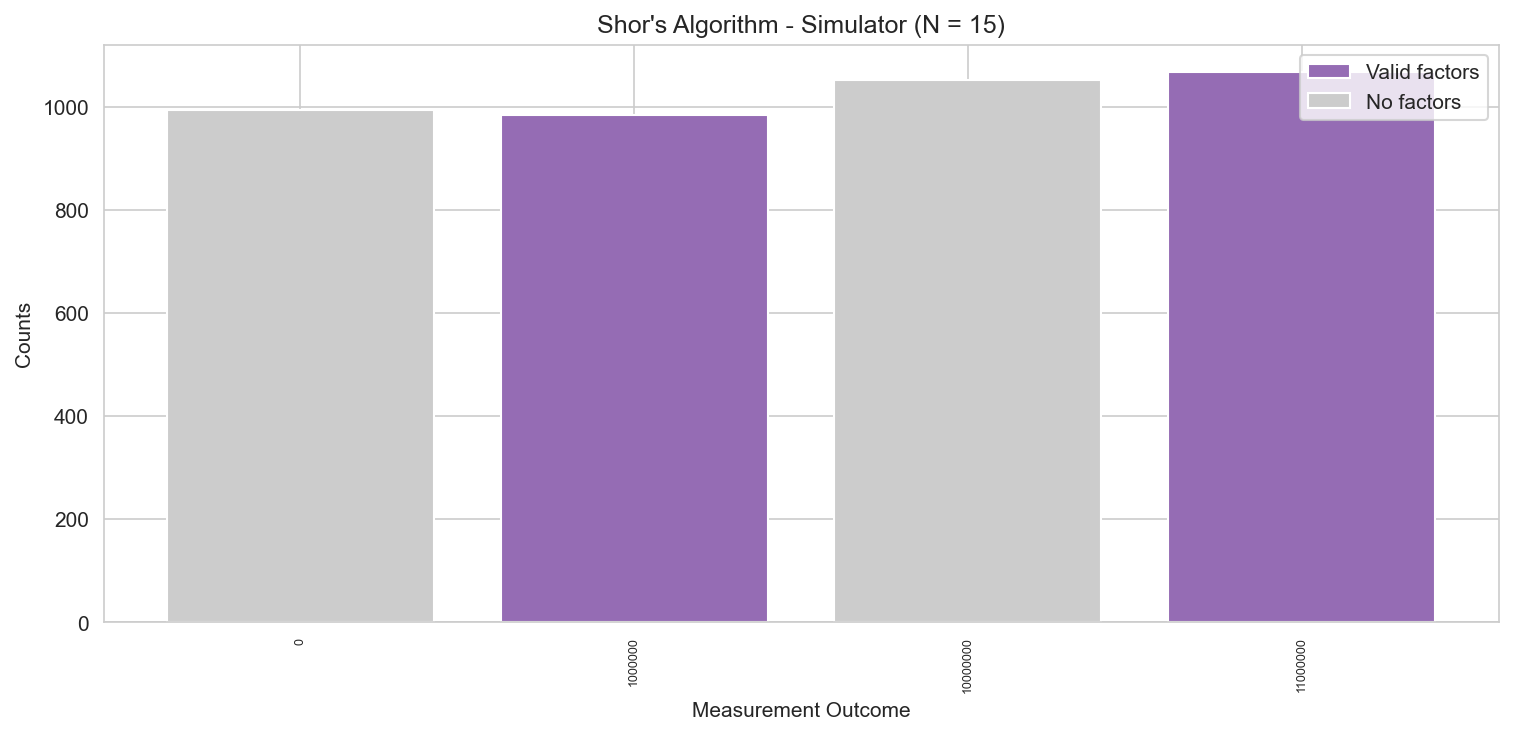
\includegraphics[width=\columnwidth]{shors_histogram_N15.png}
\caption{Measurement outcome distribution for Shor's algorithm with $N=15$, $a=7$ on the Aer simulator (4,096 shots). Purple bars indicate outcomes that yield valid factors; gray bars do not. The four sharp peaks at multiples of 64 correspond to the QFT detecting the period $r=4$.}
\label{fig:shors_n15}
\end{figure}

\subsubsection{$N = 21$, $a = 2$}

The larger circuit (15 qubits, depth 13) was executed with 4,096 shots. The expected period is $r = 6$. Since $2^{10}/6 \approx 170.67$ is not an integer, the QFT peaks are not perfectly sharp---probability leaks into neighboring states, spreading across more measurement outcomes.

Table~\ref{tab:shors21_summary} summarizes the dominant outcomes.

\begin{table}[htbp]
\caption{Shor's Algorithm: $N=21$, $a=2$ (Simulator, 4,096 shots). Selected dominant outcomes from 97 distinct measurement results.}
\label{tab:shors21_summary}
\centering
\begin{tabular}{@{}rrrrcl@{}}
\toprule
\textbf{Value} & \textbf{Count} & \textbf{Phase $\phi$} & $r_\text{cand}$ & \textbf{Valid} & \textbf{Factors} \\
\midrule
0   & 684 & 0.000 & --- & \texttimes & --- \\
512 & 684 & 0.500 & 2   & \texttimes & --- \\
341 & 501 & 0.333 & 3   & \texttimes & --- \\
171 & 490 & 0.167 & 6   & \checkmark & $(3, 7)$ \\
853 & 460 & 0.833 & 6   & \checkmark & $(3, 7)$ \\
683 & 420 & 0.667 & 3   & \texttimes & --- \\
\multicolumn{6}{@{}l}{\footnotesize + 91 additional outcomes with counts $\leq 125$} \\
\bottomrule
\end{tabular}
\end{table}

The \textbf{success rate is 32.8\%} (1,345 of 4,096 shots), correctly finding $21 = 3 \times 7$. The reduced success rate compared to $N = 15$ is attributable to two factors: (i) the non-power-of-2 period causes spectral leakage in the QFT; (ii) only phases near $\phi \approx 1/6$ and $\phi \approx 5/6$ yield the full period $r = 6$ (phases near $1/3$ and $2/3$ yield $r = 3$, which fails the period check since $2^3 = 8 \not\equiv 1 \pmod{21}$).

\subsection{Resource Extrapolation to RSA-2048}

Table~\ref{tab:extrapolation} contextualizes our results against the requirements for factoring RSA-2048.

\begin{table}[htbp]
\caption{Resource Requirements: Experimental vs.\ RSA-2048}
\label{tab:extrapolation}
\centering
\begin{tabular}{@{}lrrl@{}}
\toprule
\textbf{Target} & \textbf{Qubits} & \textbf{Success} & \textbf{Gap to HW} \\
\midrule
$N=15$ (this work) & 12     & 50.1\%  & Achievable \\
$N=21$ (this work) & 15     & 32.8\%  & Achievable \\
RSA-2048~\cite{gidney2021} & $\sim$20M & est.\ high & $\sim$20{,}000$\times$ \\
\midrule
IBM Eagle (2023) & 1{,}121 & --- & Current best \\
IBM Condor (2023) & 1{,}121 & --- & Current best \\
\bottomrule
\end{tabular}
\end{table}

\begin{figure}[htbp]
\centering
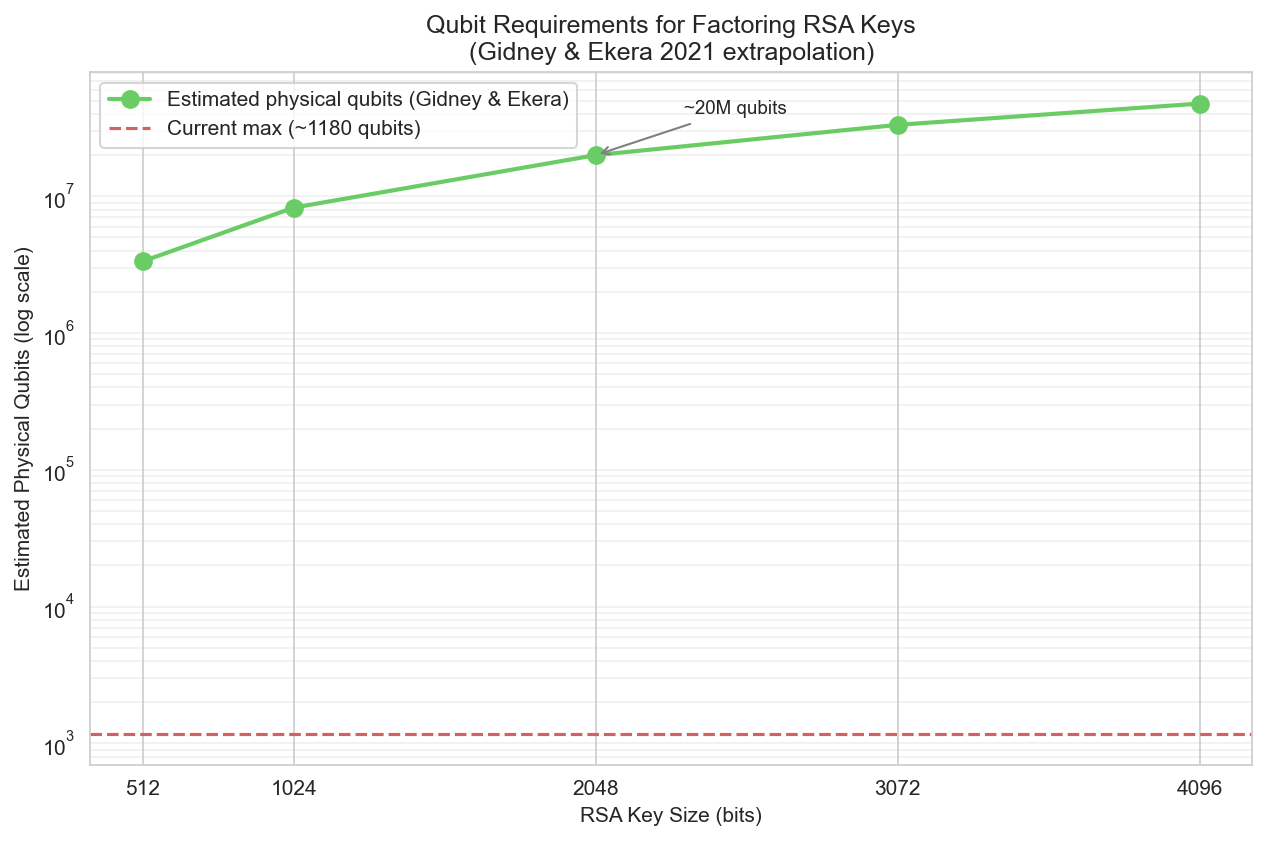
\includegraphics[width=\columnwidth]{resource_extrapolation.png}
\caption{Estimated physical qubit requirements for factoring RSA keys of increasing size (log scale). The horizontal dashed line indicates current IBM hardware ($\sim$1,100 qubits). RSA-2048 requires $\sim$20 million noisy qubits~\cite{gidney2021}, a gap of approximately four orders of magnitude.}
\label{fig:resource_extrapolation}
\end{figure}

The gap between current hardware ($\sim$1,100 qubits) and the RSA-2048 requirement ($\sim$20 million qubits)~\cite{gidney2021} is approximately four orders of magnitude in qubit count alone (Fig.~\ref{fig:resource_extrapolation}). Additionally:
\begin{itemize}[leftmargin=*]
    \item Gate error rates must improve from $\sim 10^{-3}$ to $\sim 10^{-6}$, or quantum error correction must compensate (adding $\sim$1,000$\times$ qubit overhead per logical qubit)
    \item Coherence times must sustain computation for hours, not the current millisecond regime
    \item Physical connectivity constraints require extensive SWAP gate insertion for large circuits
\end{itemize}

\subsection{ML-KEM Performance}

\subsubsection{Computational Performance}

Table~\ref{tab:mlkem_perf} presents the complete benchmark results.

\begin{table}[htbp]
\caption{ML-KEM and X25519 Performance (10,000 iterations each, Apple Silicon ARM64). All times in microseconds.}
\label{tab:mlkem_perf}
\centering
\begin{tabular}{@{}llS[table-format=3.1]S[table-format=3.1]S[table-format=3.1]S[table-format=3.1]@{}}
\toprule
\textbf{Algorithm} & \textbf{Op.} & {\textbf{Mean}} & {\textbf{Median}} & {\textbf{P95}} & {\textbf{P99}} \\
\midrule
ML-KEM-512  & KG  & 6.2  & 6.2  & 6.8  & 7.9 \\
ML-KEM-512  & Enc & 7.6  & 7.3  & 8.2  & 9.3 \\
ML-KEM-512  & Dec & 7.6  & 7.7  & 8.0  & 9.8 \\
\midrule
ML-KEM-768  & KG  & 9.8  & 9.6  & 10.4 & 12.2 \\
ML-KEM-768  & Enc & 11.1 & 11.3 & 11.6 & 14.0 \\
ML-KEM-768  & Dec & 11.6 & 11.6 & 12.5 & 14.6 \\
\midrule
ML-KEM-1024 & KG  & 13.9 & 13.9 & 14.6 & 17.3 \\
ML-KEM-1024 & Enc & 15.2 & 15.2 & 15.6 & 18.9 \\
ML-KEM-1024 & Dec & 16.7 & 16.8 & 17.3 & 19.3 \\
\midrule
X25519      & KG  & 66.4 & 66.3 & 69.0 & 74.1 \\
X25519      & Enc & 200.1 & 199.6 & 211.6 & 232.0 \\
X25519      & Dec & 132.6 & 134.4 & 143.1 & 155.1 \\
\bottomrule
\multicolumn{6}{@{}l}{\footnotesize KG = keygen, Enc = encapsulate, Dec = decapsulate.}
\end{tabular}
\end{table}

A notable result emerges: \textbf{ML-KEM-768 is significantly faster than X25519} across all operations. The speedup ratios (X25519 median / ML-KEM median) are:
\begin{itemize}[leftmargin=*]
    \item \textbf{Keygen}: $66.3 / 9.6 = 6.9\times$ faster
    \item \textbf{Encapsulation}: $199.6 / 11.3 = 17.7\times$ faster
    \item \textbf{Decapsulation}: $134.4 / 11.6 = 11.6\times$ faster
\end{itemize}

This contradicts the common assumption that post-quantum algorithms impose a computational penalty. Even ML-KEM-1024 (NIST Level 5, 256-bit security) is $4$--$13\times$ faster than X25519. Fig.~\ref{fig:mlkem_vs_x25519} visualizes this comparison for ML-KEM-768.

\begin{figure}[htbp]
\centering
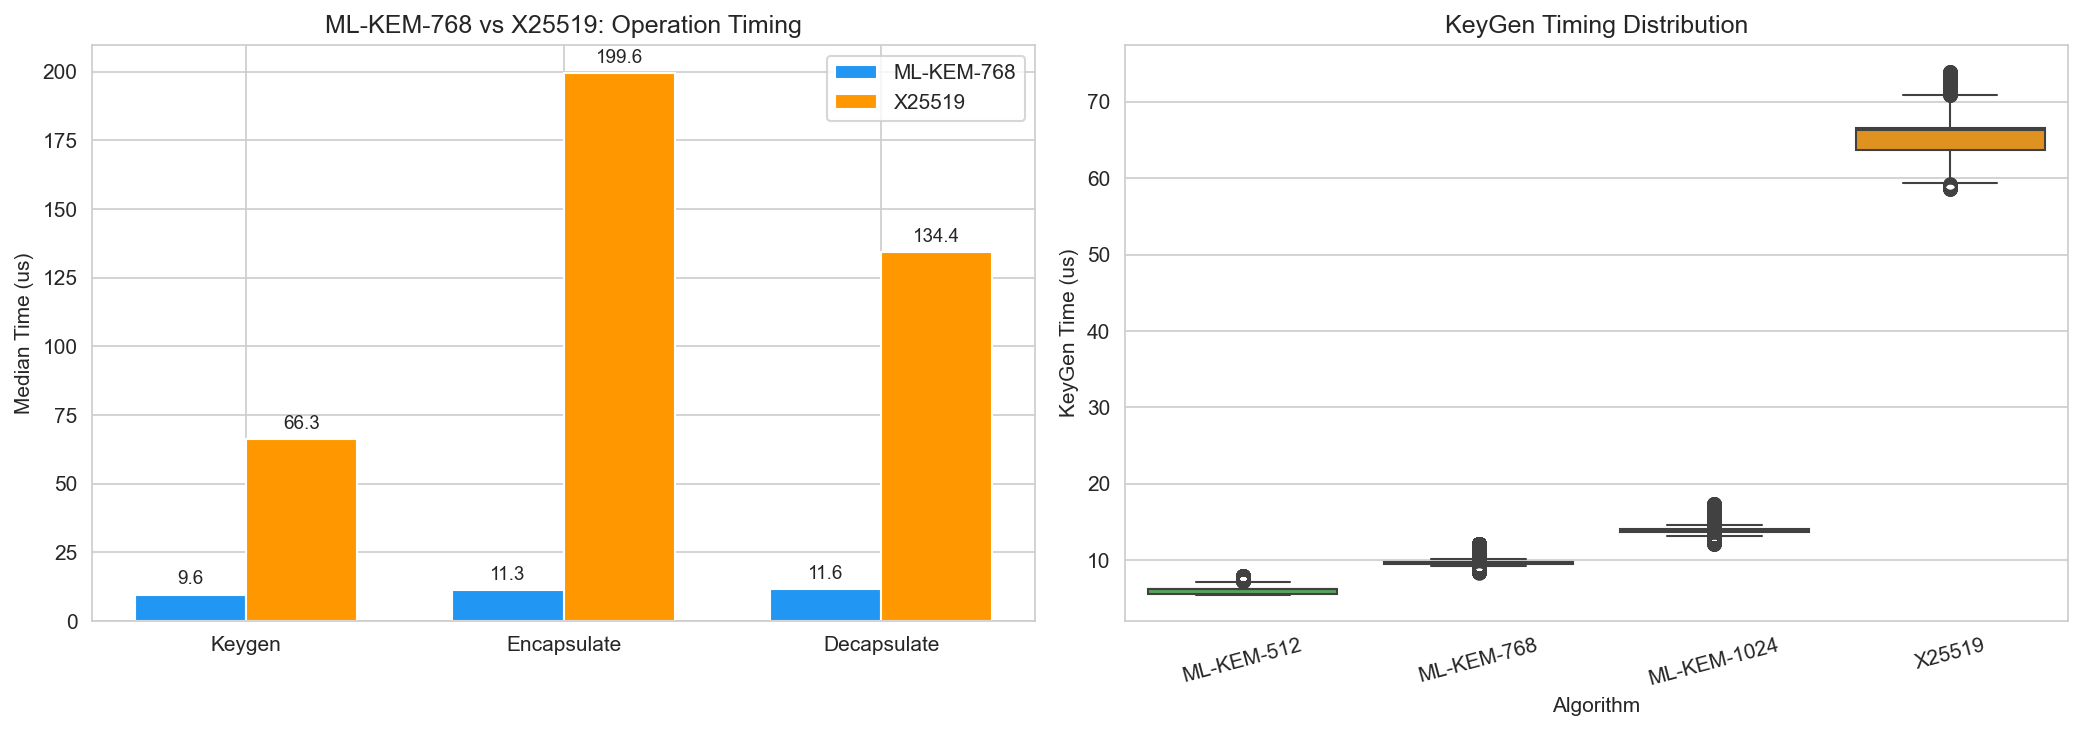
\includegraphics[width=\columnwidth]{mlkem_vs_x25519.png}
\caption{Performance comparison of ML-KEM-768 vs.\ X25519 across keygen, encapsulation, and decapsulation operations (10,000 iterations each). ML-KEM-768 is 7--18$\times$ faster across all operations.}
\label{fig:mlkem_vs_x25519}
\end{figure}

\subsubsection{Performance Scaling}

ML-KEM operations scale approximately linearly with the module rank $k$:
\begin{itemize}[leftmargin=*]
    \item ML-KEM-512 ($k=2$): $\sim$\SI{7}{\micro\second} per operation
    \item ML-KEM-768 ($k=3$): $\sim$\SI{11}{\micro\second} per operation
    \item ML-KEM-1024 ($k=4$): $\sim$\SI{15}{\micro\second} per operation
\end{itemize}

The linear scaling confirms that the NTT-based polynomial multiplication dominates the computation, and each additional module dimension adds a constant overhead.

\subsubsection{Timing Distribution}

ML-KEM operations exhibit remarkably low variance: standard deviations are consistently below \SI{1}{\micro\second} for encapsulation and decapsulation (except ML-KEM-512 encapsulation, which shows a single outlier at \SI{2905}{\micro\second}, likely from OS scheduling). In contrast, X25519 keygen has $\sigma = \SI{101}{\micro\second}$ due to variable-time scalar multiplication and occasional cache misses. This consistency is advantageous for real-time applications where worst-case latency matters.

\subsubsection{Key and Ciphertext Sizes}

\begin{table}[htbp]
\caption{Key and Ciphertext Sizes (bytes). Wire cost is the total bytes transmitted per key exchange (public key + ciphertext).}
\label{tab:sizes}
\centering
\begin{tabular}{@{}lrrrrr@{}}
\toprule
\textbf{Alg.} & \textbf{PK} & \textbf{SK} & \textbf{CT} & \textbf{SS} & \textbf{Wire} \\
\midrule
X25519      & 32    & 32    & 32    & 32 & 64 \\
ML-KEM-512  & 800   & 1{,}632 & 768   & 32 & 1{,}568 \\
ML-KEM-768  & 1{,}184 & 2{,}400 & 1{,}088 & 32 & 2{,}272 \\
ML-KEM-1024 & 1{,}568 & 3{,}168 & 1{,}568 & 32 & 3{,}136 \\
\bottomrule
\multicolumn{6}{@{}l}{\footnotesize PK = public key, SK = secret key, CT = ciphertext, SS = shared secret.}
\end{tabular}
\end{table}

\begin{figure}[htbp]
\centering
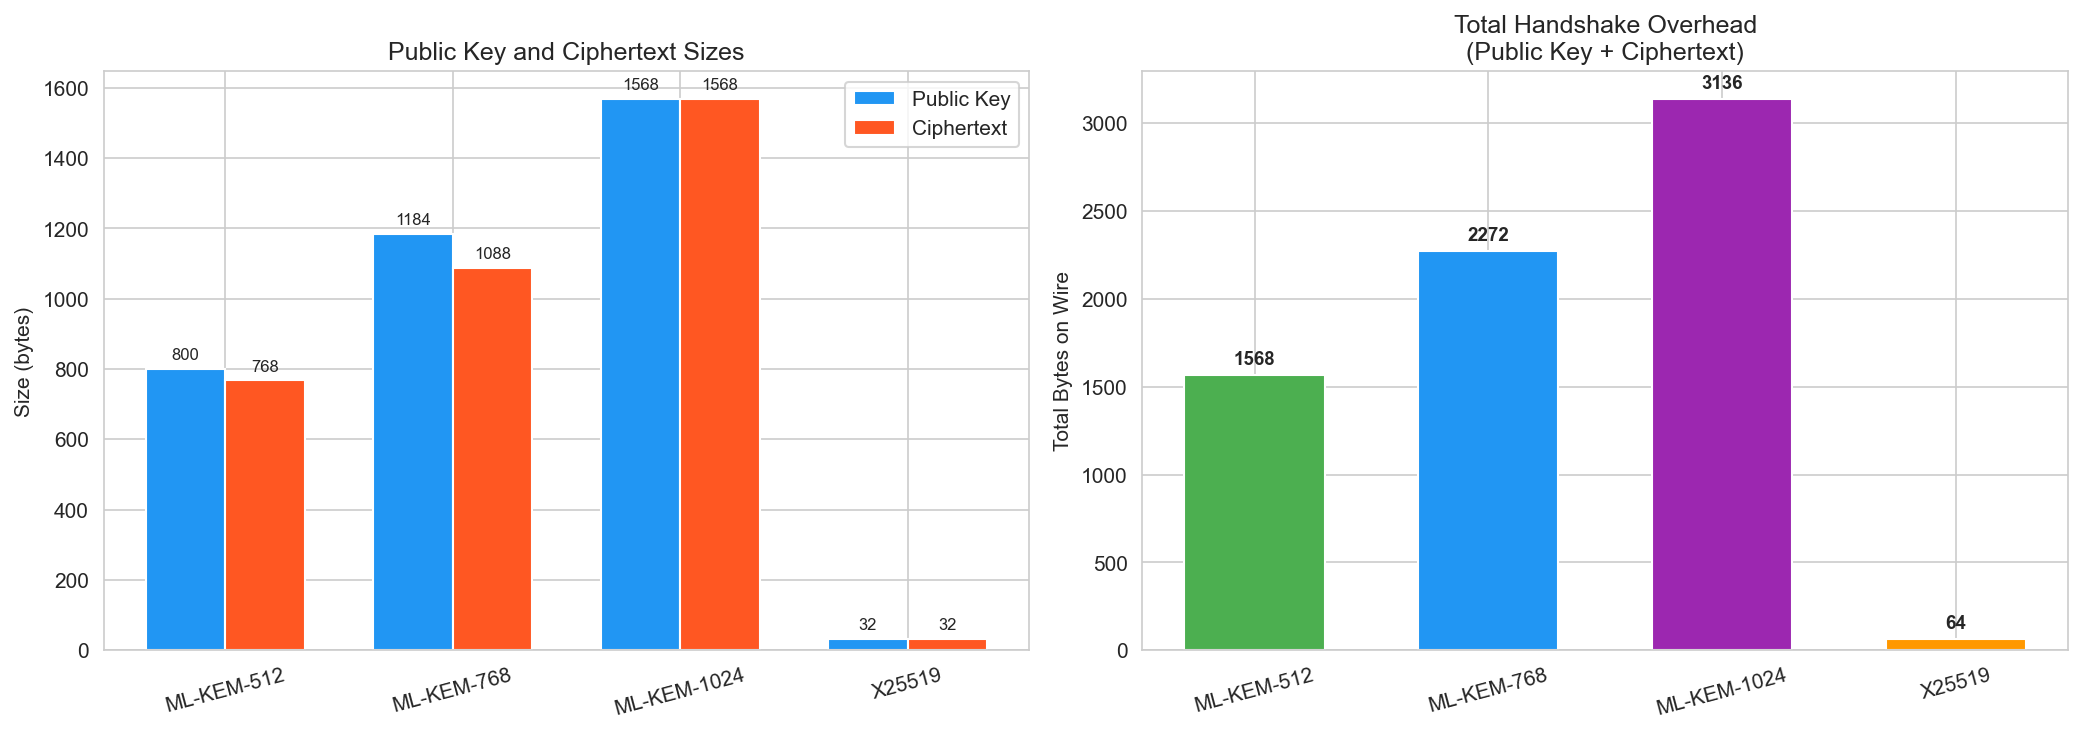
\includegraphics[width=\columnwidth]{size_comparison.png}
\caption{Key and ciphertext sizes across algorithms. ML-KEM keys and ciphertexts are 25--50$\times$ larger than X25519, but the absolute overhead ($\sim$2~KB) is modest for most applications.}
\label{fig:size_comparison}
\end{figure}

ML-KEM-768 requires transmitting 2,272 bytes vs.\ X25519's 64 bytes---a $35\times$ increase (Fig.~\ref{fig:size_comparison}). While the size difference is significant in relative terms, the absolute overhead of $\sim$\SI{2}{\kilo\byte} per key exchange is modest in context:
\begin{itemize}[leftmargin=*]
    \item A TLS 1.3 ClientHello adds $\sim$\SI{2}{\kilo\byte}, fitting within two TCP segments
    \item A typical HTTPS page load transfers 2--5 MB; the PQC overhead is $<0.1\%$
    \item For bandwidth-constrained IoT, the overhead may require protocol-level optimization
\end{itemize}

%======================================================================
\section{Discussion}
\label{sec:discussion}

\subsection{Threat Assessment}

Our experiments confirm that Shor's algorithm is correct and implementable on current quantum computing frameworks. The 50.1\% success rate for $N=15$ precisely matches the theoretical expectation: of four QFT peaks, two ($\phi = 1/4$ and $\phi = 3/4$) yield the full period $r = 4$, while $\phi = 0$ is trivial and $\phi = 1/2$ yields a period divisor. The degradation to 32.8\% for $N=21$ is due to spectral leakage from the non-power-of-2 period, not hardware noise---the simulator is noiseless.

The significance of our simulator results is that they establish a \emph{lower bound} on the algorithm's correctness: any failure on real hardware beyond these rates is attributable to noise, not algorithmic error. Published hardware demonstrations of Shor's algorithm for small numbers~\cite{vandersypen2001} have historically shown significant degradation due to decoherence and gate errors, consistent with NISQ-era limitations~\cite{preskill2018}.

The RSA-2048 gap remains vast: $\sim$20,000$\times$ in qubit count, $\sim$1,000$\times$ in error rate, and orders of magnitude in coherence time. Even with optimistic projections, CRQCs are estimated to be 15--30 years away~\cite{mosca2018}. However, the HNDL threat means that data encrypted today with RSA or ECDH may be compromised retroactively.

\subsection{Defense Readiness}

\textbf{Computational cost is negative.} Our finding that ML-KEM-768 is 7--18$\times$ faster than X25519 on Apple Silicon is attributable to:
\begin{enumerate}[leftmargin=*]
    \item \textbf{NTT-based arithmetic}: ML-KEM's core operations use the Number Theoretic Transform over $\mathbb{Z}_{3329}[X]/(X^{256}+1)$, which decomposes into cache-friendly, vectorizable butterfly operations
    \item \textbf{No big-integer arithmetic}: Unlike RSA's modular exponentiation or X25519's scalar multiplication on a 255-bit curve, ML-KEM operates on fixed-size 16-bit coefficients
    \item \textbf{Constant-time by design}: ML-KEM's operations have inherently data-independent timing, avoiding the variable-time patterns that increase X25519's variance
\end{enumerate}

This speedup is consistent with other platform benchmarks~\cite{bos2018} and suggests that PQC migration may actually \emph{improve} server-side throughput for applications performing many key exchanges.

\textbf{Size cost is modest but real.} The $35\times$ increase in wire cost (Table~\ref{tab:sizes}) is the primary tangible cost of migration. For most web and API applications, the additional $\sim$\SI{2}{\kilo\byte} per handshake is negligible. For constrained environments (low-bandwidth IoT, satellite links, smart cards with limited memory), the larger keys and ciphertexts may require protocol adaptation.

\subsection{Migration Implications}

NIST has published concrete deprecation timelines~\cite{nistir8547}: RSA-2048 and 112-bit security to be deprecated by 2030 and disallowed by 2035 for federal use. The recommended migration path is \emph{hybrid key exchange}---combining ML-KEM-768 with X25519~\cite{langley2024}---which maintains security even if one algorithm is later found vulnerable. This approach is already deployed in Chrome and Firefox.

Given our findings:
\begin{enumerate}[leftmargin=*]
    \item The computational cost of ML-KEM is zero or negative (it's faster)
    \item The bandwidth cost is $\sim$\SI{2}{\kilo\byte} per exchange (negligible for most applications)
    \item The HNDL threat creates urgency independent of CRQC timelines
\end{enumerate}
The primary barrier to migration is ecosystem readiness, not performance.

%======================================================================
\section{Limitations}
\label{sec:limitations}

\begin{enumerate}[leftmargin=*]
    \item \textbf{Small factoring instances}: Our Shor's implementation is limited to $N \in \{15, 21\}$, which are far from cryptographically relevant. The modular exponentiation circuits use hardcoded permutations rather than general modular arithmetic.
    \item \textbf{Simulator only}: Due to IBM Quantum Platform's migration from the legacy API to IBM Cloud during the course of this work, we were unable to obtain hardware results. Our simulator results establish algorithmic correctness but do not capture the effects of real quantum noise.
    \item \textbf{Single platform}: ML-KEM benchmarks are from Apple Silicon (ARM64) only. Performance on x86-64 (with AVX2/AVX-512), server-class ARM, and embedded platforms may differ.
    \item \textbf{Library-level measurement}: We benchmark through Python bindings (liboqs-python), which add overhead vs.\ native C. Absolute timings may be faster in production deployments.
    \item \textbf{No protocol integration}: We measure primitive-level performance, not end-to-end protocol impact (TLS handshake latency, certificate chain size with PQ signatures, etc.).
\end{enumerate}

%======================================================================
\section{Conclusion and Future Work}
\label{sec:conclusion}

We presented an empirical study bridging both sides of the quantum cryptographic challenge. On the threat side, Shor's algorithm successfully factors $N=15$ (50.1\% success) and $N=21$ (32.8\%) on a quantum simulator, validating the algorithmic threat, while RSA-2048 remains $\sim$20,000$\times$ beyond current hardware capabilities. On the defense side, ML-KEM-768 is 7--18$\times$ faster than X25519 across all operations, with the primary cost being a $35\times$ increase in key/ciphertext sizes ($\sim$\SI{2}{\kilo\byte} per exchange).

Our integrated analysis leads to a clear conclusion: \textbf{the quantum threat is real but distant, the defense is ready and fast, and the migration cost is minimal.} Under the HNDL threat model, organizations handling long-lived sensitive data should begin migrating to post-quantum key exchange now, using hybrid ML-KEM + X25519 deployments as a transition strategy.

Future work includes: (i) hardware execution of Shor's on IBM Cloud Quantum when platform access is restored; (ii) benchmarking ML-DSA and SLH-DSA post-quantum signatures; (iii) cross-platform benchmarks on x86-64 and embedded ARM; (iv) end-to-end TLS 1.3 handshake measurements with PQ key exchange; and (v) extending Shor's to larger instances using iterative phase estimation to reduce qubit requirements.

\subsection*{Reproducibility}

All code, data, and analysis are publicly available at \url{https://github.com/utkarshc-sudo/btech-pqc-shors}, with pinned dependency versions and automated Makefile targets for full reproduction.

\bibliographystyle{IEEEtran}
\bibliography{references}

\end{document}
